%-----------------------------------------------------------------------------------------------------------------------------------------------%
%	The MIT License (MIT)
%
%	Copyright (c) 2021 Jitin Nair
%
%	Permission is hereby granted, free of charge, to any person obtaining a copy
%	of this software and associated documentation files (the "Software"), to deal
%	in the Software without restriction, including without limitation the rights
%	to use, copy, modify, merge, publish, distribute, sublicense, and/or sell
%	copies of the Software, and to permit persons to whom the Software is
%	furnished to do so, subject to the following conditions:
%	
%	THE SOFTWARE IS PROVIDED "AS IS", WITHOUT WARRANTY OF ANY KIND, EXPRESS OR
%	IMPLIED, INCLUDING BUT NOT LIMITED TO THE WARRANTIES OF MERCHANTABILITY,
%	FITNESS FOR A PARTICULAR PURPOSE AND NONINFRINGEMENT. IN NO EVENT SHALL THE
%	AUTHORS OR COPYRIGHT HOLDERS BE LIABLE FOR ANY CLAIM, DAMAGES OR OTHER
%	LIABILITY, WHETHER IN AN ACTION OF CONTRACT, TORT OR OTHERWISE, ARISING FROM,
%	OUT OF OR IN CONNECTION WITH THE SOFTWARE OR THE USE OR OTHER DEALINGS IN
%	THE SOFTWARE.
%
%-----------------------------------------------------------------------------------------------------------------------------------------------%

%----------------------------------------------------------------------------------------
%	DOCUMENT DEFINITION
%----------------------------------------------------------------------------------------

\documentclass[a4paper,11pt]{article}

%----------------------------------------------------------------------------------------
%	PACKAGES
%----------------------------------------------------------------------------------------
\usepackage{url}
\usepackage{parskip}
\usepackage[usenames,dvipsnames]{xcolor}
\usepackage[scale=0.9]{geometry}
\usepackage{tabularx}
\usepackage{enumitem}
\usepackage{titlesec}
\usepackage{fontawesome5}
\usepackage{graphicx}
\usepackage[unicode, draft=false]{hyperref}

%----------------------------------------------------------------------------------------
%	FORMATTING
%----------------------------------------------------------------------------------------

% centered version of 'X' col. type
\newcolumntype{C}{>{\centering\arraybackslash}X} 

% custom section formatting
\titleformat{\section}{\Large\scshape\raggedright}{}{0em}{}[\titlerule]
\titlespacing{\section}{0pt}{8pt}{8pt}

% hyperref setup
\usepackage[unicode, draft=false]{hyperref}
\definecolor{linkcolour}{rgb}{0,0.2,0.6}
\hypersetup{colorlinks,breaklinks,urlcolor=linkcolour,linkcolor=linkcolour}

% job listing environments
\newenvironment{joblong}[2]
    {
    \begin{tabularx}{\linewidth}{@{}l X r@{}}
    \textbf{#1} & \hfill &  #2 \\[3.75pt]
    \end{tabularx}
    \begin{minipage}[t]{\linewidth}
    \begin{itemize}[nosep,after=\strut, leftmargin=1em, itemsep=3pt,label=--]
    }
    {
    \end{itemize}
    \end{minipage}    
    }

%----------------------------------------------------------------------------------------
%	BEGIN DOCUMENT
%----------------------------------------------------------------------------------------
\begin{document}

\pagestyle{empty} 
\vspace*{-1.5cm}

%----------------------------------------------------------------------------------------
%	TITLE WITH PHOTO
%----------------------------------------------------------------------------------------

\begin{tabularx}{\linewidth}{@{} X r @{}}
\begin{minipage}[t]{0.7\linewidth}
\vspace{0.4cm}
{\Huge\bfseries\sffamily Alain CHENG} \\[12pt]
\href{mailto:Alain.cheng@protonmail.com}{\raisebox{-0.05\height}\faEnvelope\ Alain.cheng@protonmail.com} \ $|$ \ 
\href{https://github.com/cheng-alain}{\raisebox{-0.05\height}\faGithub\ cheng-alain} \\[3pt]
\href{https://www.linkedin.com/in/alain-cheng}{\raisebox{-0.05\height}\faLinkedin\ alain-cheng} \ $|$ \ 
\href{https://portfolio-url.com}{\raisebox{-0.05\height}\faGlobe\ portfolio} \ $|$ \ 
\href{tel:+33650425904}{\raisebox{-0.05\height}\faMobile\ 06.50.42.59.04}
\end{minipage}
&
\begin{minipage}[t]{0.25\linewidth}
\vspace{0pt}
\raggedleft
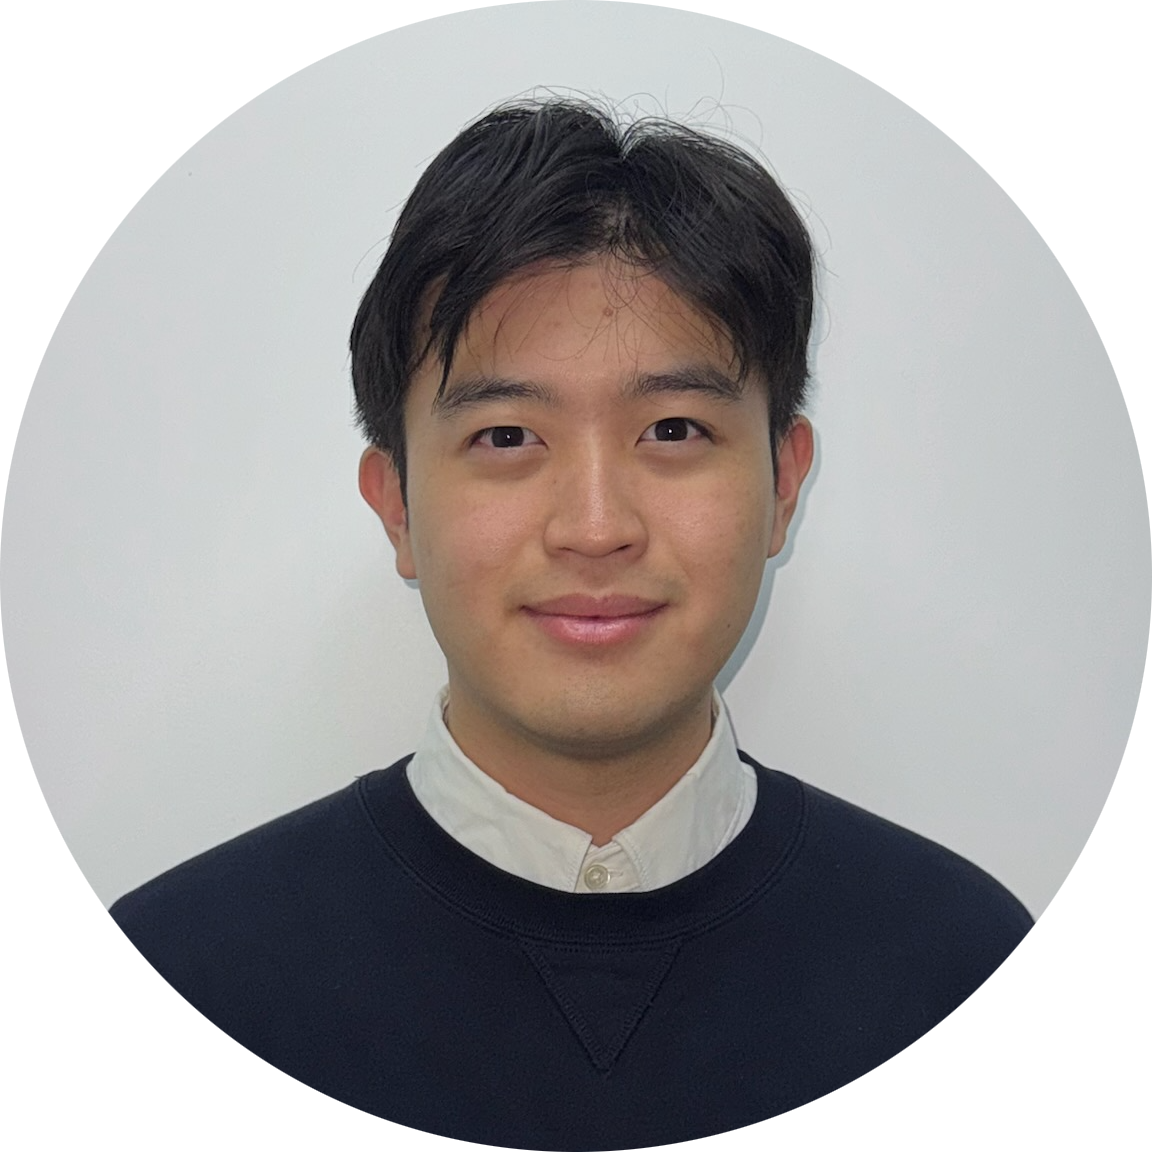
\includegraphics[width=3.2cm,height=3.2cm,keepaspectratio]{images/photo.png}
\end{minipage}
\\[15pt]
\end{tabularx}

%----------------------------------------------------------------------------------------
%	SECTIONS
%----------------------------------------------------------------------------------------

\section{Profil}
Ingénieur DevOps Passionné par l'automatisation et l'infrastructure cloud, je conçois et maintiens des environnements DevOps robustes et scalables.

\section{Compétences Techniques}
\begin{tabularx}{\linewidth}{@{}l X@{}}
\textbf{Cloud \& Infrastructure} & AWS, Azure, Kubernetes, Docker, Helm, Linux \\[3pt]
\textbf{IaC \& CI/CD} & Terraform, Ansible, GitLab/GitHub Actions, GitOps (ArgoCD) \\[3pt]
\textbf{Monitoring \& Observabilité} & Prometheus, Grafana, ELK Stack \\[3pt]
\textbf{Développement \& Scripting} & Golang, Python, Bash, PowerShell, YAML, API REST \\[3pt]
\textbf{Sécurité \& Réseau} & Vault, SSL/TLS, Load balancing (Traefik), LDAP/SSO \\[3pt]
\end{tabularx}

\section{Expérience Professionnelle}

\begin{joblong}{Ingénieur DevOps / SysOps - Flaminem}{Sep 2023 - Sep 2025}
\item Développement et maintenance de rôles Ansible pour automatisation complète des déploiements
\item Création et déploiement de charts Helm personnalisés (GLPI, Diun, Glauth)
\item Surveillance des plateformes avec outils de monitoring (Prometheus/Grafana)
\item Administration et optimisation des chaînes GitLab CI/CD et runners
\item Implémentation architecture SSO complète avec backend LDAP et intégration applications métier
\item Support technique équipes développement : débogage containers, accès ressources, dépannage réseau
\end{joblong}

\begin{joblong}{Administrateur Système - Ad Education}{Oct 2022 - Sep 2023}
\item Gestion de l'Active Directory
\item Administration, Gestion à distance des bornes WiFi Cisco Meraki
\item Planifications de mise en place d'infrastructures réseaux sur divers sites distants (Baies de brassage, Serveurs, Routeur, Switch...)
\item Résolution incidents système/réseau avec gestion de tickets
\end{joblong}
  
\section{Projets}

\begin{tabularx}{\linewidth}{ @{}l r@{} }
\textbf{Infrastructure DevOps AudioProthèse+} & \hfill \href{https://github.com/cheng-alain}{Projet d'études M2} \\[3.75pt]
\multicolumn{2}{@{}X@{}}{Architecture DevOps complète pour réseau de 50+ centres d'audioprothèse avec conformité RGPD. Automatisation des déploiements, mise en place d'observabilité centralisée, et optimisation des coûts par mutualisation des ressources cloud.}  \\
\end{tabularx}

\begin{tabularx}{\linewidth}{ @{}l r@{} }
\textbf{CLI d'Authentification Golang} & \hfill \href{https://github.com/cheng-alain}{Projet d'études M1} \\[3.75pt]
\multicolumn{2}{@{}X@{}}{Interface ligne de commande en Go pour intégration de solutions d'authentification modernes. Implémentation de la gestion utilisateurs et permissions via API REST avec tests unitaires complets.}  \\
\end{tabularx}

\begin{tabularx}{\linewidth}{ @{}l r@{} }
\textbf{Homelab Kubernetes sur Raspberry Pi} & \hfill \href{https://github.com/cheng-alain}{Homelab} \\[3.75pt]
\multicolumn{2}{@{}X@{}}{Cluster Kubernetes mono-nœud sur Raspberry Pi hébergeant portfolio personnel, CI/CD, monitoring et stockage distribué. Plateforme d'expérimentation pour tester différentes stacks open source DevOps.}  \\
\end{tabularx}

\section{Formation}
\begin{tabularx}{\linewidth}{@{}l X@{}}	
2023 - 2025 & Master DevOps - \textbf{SUP DE VINCI ISI PARIS} \\
\end{tabularx}

\end{document}